%!TEX root = ../Report.tex
%************************************************

% Conceptual design

\chapter{Introduction}
In this part of the document a conceptual design is proposed to solve the problem of composing music algorithmically.
Composing music algorithmically can be done in a variety of ways. Different types of algorithms can be utilized:
\begin{itemize}
\item Algorithms that utilize expert knowledge. Expert systems utilize knowledge from a specific domain in order to make decisions.
\item Algortihms that learn. These algorithms utilize pattern recognition to learn from data in order to make decisions.
\end{itemize}
For an expert system to be used in algorithmic music composition knowledge from music theory is utilized in order for the algorithm to make decisions. When too many constraints are imposed on the algorithm the variety of the type of music produced is lessened.

For this project however, the focus is on algorithms that can learn. In order to design an application that utilizes machine learning algorithms to compose music the project will first be decomposed into discrete units. The function and interaction of each unit will be investigated. 

Different types of machine learning algorithms will be investigated and the best solution will be chosen that satisfies the requirements of the project.

\chapter{System architecture}
In this section the project will be broken down into discrete functional components and the interaction between different components will be investigated.
\\\\
Figure \ref{ims:oppflow} shows the interaction of the user with the application. 
The user interacts with the application and selects a certain style of music to be composed. The application generates the music according to a certain algorithm and plays back the generated piece. 
\\\\
Figure \ref{ims:conceptuserinterface} indicates a conceptual user interface with the primary elements. A user is able to select a certain style of music for composition. Once the piece is generated the user is able to save the music to a \ac{MIDI} file.
\\\\
The core functionality of the application resides in the algorithm that is responsible for composing a piece of music.

\begin{figure}
\centerline{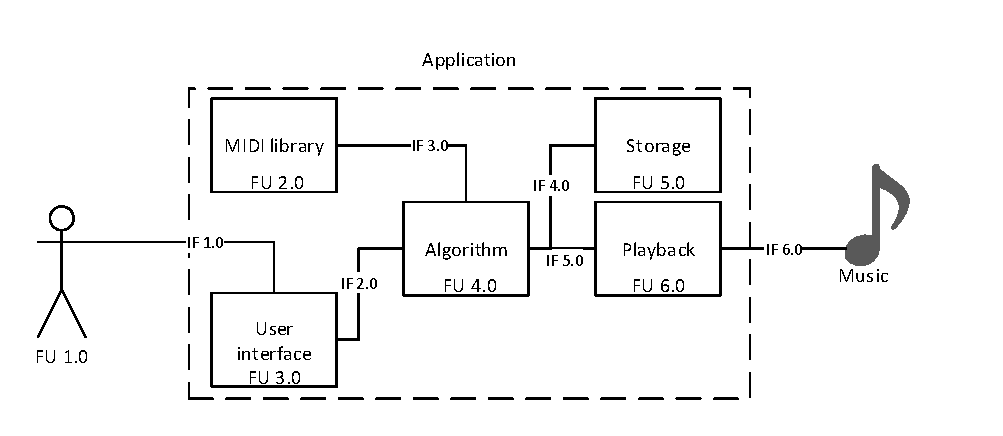
\includegraphics[width=400px]{../images/architecture.pdf}}
\caption{Functional architecture}
\label{ims:funcarch}
\end{figure}

By incorporating all these elements we can concretely describe the project in discrete components in a functional architecture diagram, see figure \ref{ims:funcarch}.

\section{Functional architecture}
\subsection{Functional Unit 1 - Operator}
The operator is responsible for interacting with the application. The operator will select the style or category for composition and instruct to application to compose music.
If a certain piece of music is to be save the operator will be responsible for instructing the application to do so and to select the location the \ac{MIDI} file is to be saved

\subsection{Functional Unit 2 - MIDI library }
The MIDI library is a large collection of \ac{MIDI} files. The files in the \ac{MIDI} library are organized into categories. Each category represents a certain style of music
The algorithm will utilize a subset of the library (a category) as input.

\subsection{Functional Unit 3 - User Interface}
The user interface is the front end of the application. The operator interacts with this functional unit in order to instruct the application what to do.

The user interface should be designed in a user-friendly manner in order to accommodate the operator.
A conceptual user interface is shown in figure \ref{ims:conceptuserinterface}. 

This user interface allows the user to select a certain style, instruct the algorithm to compose music and to save or play back a piece of music once it is composed.

\subsection{Functional Unit 4 - Algorithm}
The algorithm is the central part of this project. The algorithm converts the input \acp{MIDI} into output \ac{MIDI}.

The algorithm will utilize a category of \ac{MIDI} files from the \ac{MIDI} library in order to compose a new piece of music not in the \ac{MIDI} library.

The output piece of music will represent the style of music that was used as input.
The possible types of algorithms were discussed in section \label{chap:comp_algo}

\subsection{Functional Unit 5 - Storage}
This unit is responsible for storing the output \ac{MIDI} from the algorithm into a \ac{MIDI} file.

\subsection{Functional Unit 6 - Playback}
This unit is responsible for playing back the output \ac{MIDI} from the algorithm through an audio output device

\section{Interfaces}
The interfaces indicate the interaction between different functional units.
The interfaces have the following functions:
\\Interface:
\begin{enumerate}
\item Interface between the user and the user interface. This input would be from a input peripheral device.
\item Interface between the user interface and the algorithm. The interface calls the algorithm with the parameters supplied by the user such as when to start and what type of style was selected
\item Interface between the \ac{MIDI} library and the algorithm. The input to the algorithm is a selection of \acp{MIDI}. The interface converts \ac{MIDI} files into a format required by the algorithm
\item Interface between the algorithm and storage. This interface converts the output from the algorithm into the \ac{MIDI} file format
\item Interface between the algorithm and playback. This interface converts the output from the algorithm into a format that is ready for playback through the playback functional unit.
\item Interface between the playback and the music. This represents the audio output device and it's workings.
\end{enumerate}

\chapter{Operational Flow}

The operational flow indicates the interaction between the operator and the application and how the operator should use it.

\begin{figure}[ht]
\centerline{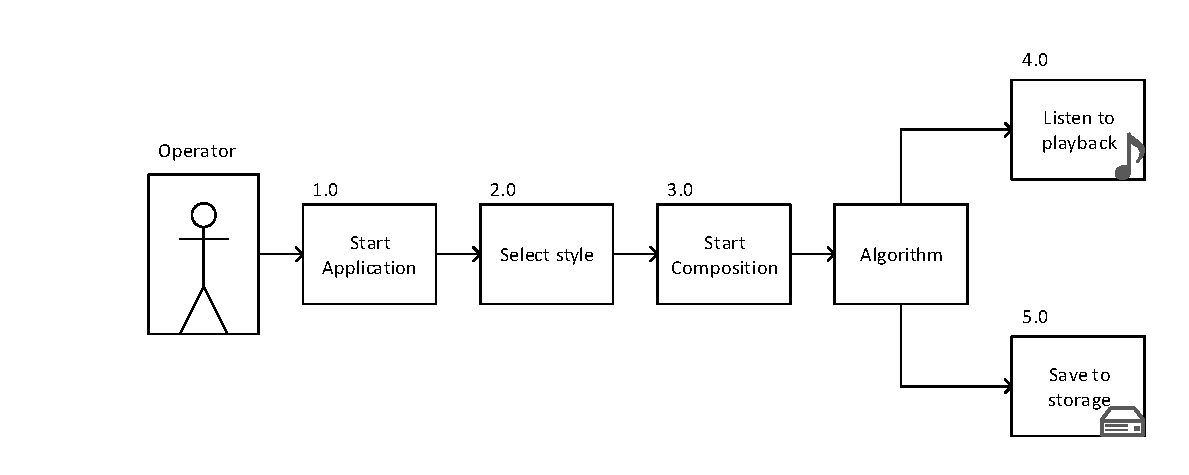
\includegraphics[width=400px]{../images/operational_flow.pdf}}
\caption{Operational Flow}
\label{ims:oppflow}
\end{figure}

\begin{figure}[ht]
\centerline{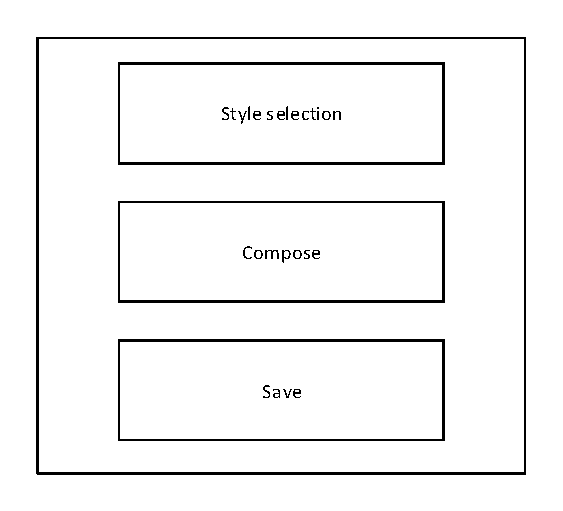
\includegraphics[width=150px]{../images/user_interface.pdf}}
\caption{Conceptual user interface}
\label{ims:conceptuserinterface}
\end{figure}

Figure \ref{ims:oppflow} shows how the operator interacts with the application. Figure \ref{ims:conceptuserinterface} shows a conceptual user interface with which the operator would interact.

For this application, the operator selects the style of music to be composed; instructs the application to compose the music according to the selected style and then to instruct the application to either play back the piece of generated music or save it to storage.

\chapter{Conclusion}
In order to solve the problem of generating music algorithmically the task was broken down into its functional architecture. From this each functional unit and its interaction is made apparent. The core component of this project is the algorithm which is used to compose music